\documentclass[11pt, a4paper]{article}
\usepackage[left=1.4cm,text={18.2cm, 25.2cm},top=2.3cm]{geometry}

\usepackage{times}
\usepackage[czech]{babel}
\usepackage[IL2]{fontenc}
\usepackage[utf8]{inputenc}
\usepackage{listings}

\usepackage{amsmath, amsthm, amssymb}
\usepackage[bottom]{footmisc}
\usepackage{graphicx}
\usepackage{hyperref}
\usepackage{geometry}
\geometry{a4paper}

\begin{document}

\begin{titlepage}
\thispagestyle{empty}

    \begin{center}

        {\Huge \textsc{Vysoké učení technické v~Brně \\[0.5em]}}

        {\huge \textsc{Fakulta informačních technologií}}

        \vspace{\stretch{0.382}}

        {\Large Mikroprocesorové a vstavané systémy \\[0.5em]
        \LARGE Digitálne FM rádio
         }

        \vspace{\stretch{0.618}}

    \end{center}
{\Large 2024 \hfill Boris Hatala (xhatal02)}

\end{titlepage}

\newpage
\tableofcontents
\newpage


\section{Úvod}
Táto dokumentácia opisuje návrh a implementáciu digitálneho FM rádia postaveného 
na hardvéri ESP32 a ďalších súčastiach.

\subsection{Cieľ projektu}
Cieľom je vytvoriť funkčné digitálne FM rádio, 
ktoré umožňuje používateľovi nastavovať frekvenciu v pásme 76MHz až 108Mhz FM a 
ovládať hlasitosť.

\section{Použité metódy a technológie}
V tejto časti je uvedený použitý hardvér a knižnice, ktoré umožnili vypracovanie projektu. 
Program je napísaný v jazyku C++ vo vývojovm prostredí Arduino IDE. \footnote{\url{https://www.arduino.cc/en/software}}

\subsection{Hardvér}
\begin{itemize}
    \item Doska ESP32 Wemos D1 R32\footnote{\url{https://docs.platformio.org/en/latest/boards/espressif32/wemos_d1_uno32.html}}
    \item Modul s OLED displejom 0,96`` \-\ Adafruit\footnote{\url{https://www.hadex.cz/m508a-displej-oled-096-128x64-znaku-7pinu-bily/}}
    \item FM príjmač na bázi čipsetu RDA5807M\footnote{\url{https://www.hadex.cz/m501a-fm-prijimac-pro-arduino-modul-rrd102-v20-io-rda5807m/}}
    \item Audio zosilovač PAM8407D\footnote{\url{https://www.diodes.com/assets/Datasheets/products_inactive_data/PAM8407.pdf}}
    \item Rotačný enkodér KY-040\footnote{\url{https://elty.pl/cs_CZ/p/Impulsni-modul-snimace-KY-040/1155}}
\end{itemize}
\subsection{Knižnice}
\begin{itemize}
    \item Wire 
    \item Adafruit GFX \footnote{\url{https://github.com/adafruit/Adafruit-GFX-Library}}
    \item Adafruit SSD1306 \footnote{\url{https://github.com/adafruit/Adafruit_SSD1306}}
    \item PU2CLR RDA5807 \footnote{\url{https://github.com/pu2clr/RDA5807}} 
    \item KY040-rotary \footnote{\url{https://github.com/dmachard/KY040-rotary}} 
\end{itemize}

\section{Použitie}
Pri zapojení rádia sa inicializujú všetky komponenty a rádio začne hrať na predom
určenej frekvenci v programe 106,50 MHz. Otočným enkóderom sa 
dá meniť frekvencia a stlačením tlačidla na enkóderi sa dá prepínať medzi 
režimom nastavovania frekvencie a hlasitosti. Aktuálne nastavenia sa zobrazujú 
na OLED displeji.

Ukážka použita: \-\ \url{https://drive.google.com/file/d/1KT2sNgN7PxN1Bjnalx79Aksi3KVg7GT5/view?usp=sharing}

\section{Implementačné detaily}
Táto kapitola popisuje zapojenie jednotlivých komponentov a ich spracovanie v programe.

\subsection{Zapojenie}
\begin{figure}[h!]
\centering
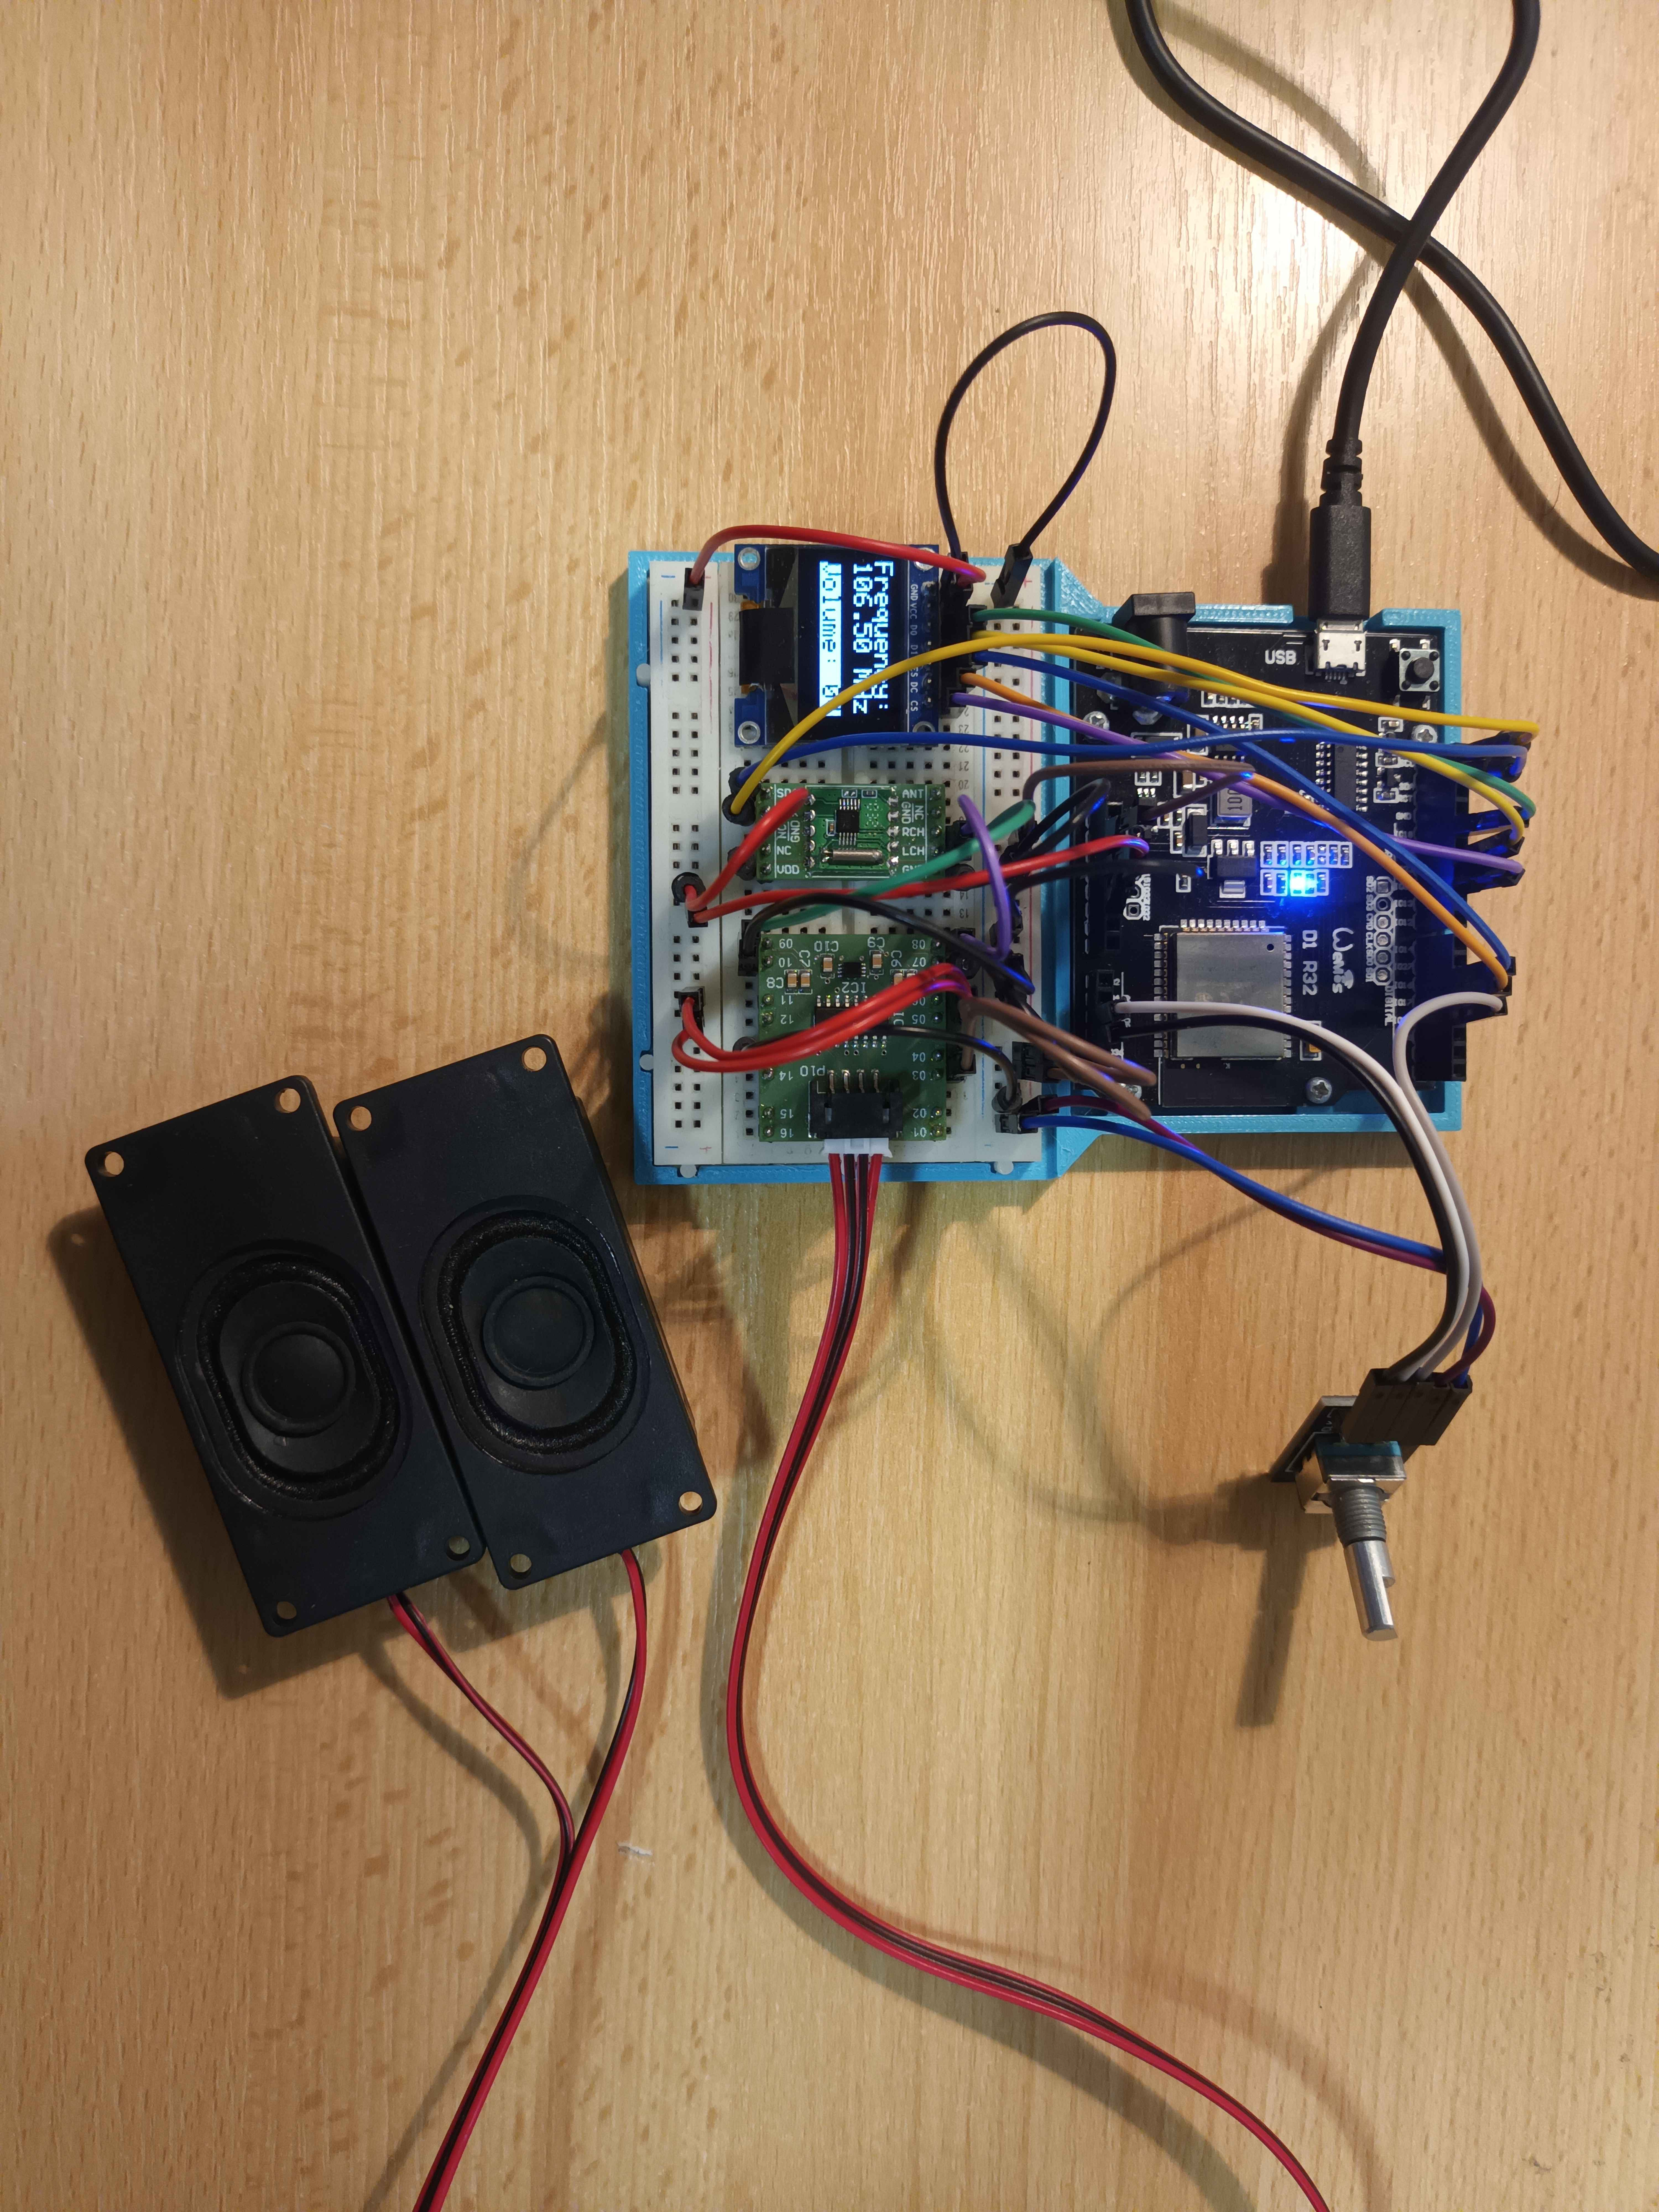
\includegraphics[width=0.6\textwidth, angle=90]{zapojenie.jpg}
\caption{Zapojenie rádia}
\end{figure}
\subsubsection{Zapojenie FM modulu RDA5807M a OLED displeja}

\begin{minipage}[t]{0.48\textwidth}
\centering
\textbf{FM modul RDA5807M}
\begin{tabular}{|c|c|c|}
    \hline
    \textbf{FM Pin} & \textbf{ESP32 Pin} & \textbf{PAM8407 Pin} \\
    \hline
    VDD & 3.3V & -- \\
    GND & GND & -- \\
    SDA & GPIO21 (SDA) & -- \\
    SCK & GPIO22 (SCL) & -- \\
    RCH & -- & 08 \\
    LCH & -- & 09 \\
    ANT & Drôtová anténa & -- \\
    NC\textbar GND & -- & -- \\
    NC\textbar GND & -- & --\\
    \hline
\end{tabular}
\end{minipage}
\hfill
\begin{minipage}[t]{0.48\textwidth}
\centering
\textbf{OLED displej Adafruit}
\begin{tabular}{|c|c|}
    \hline
    \textbf{OLED Pin} & \textbf{ESP32 Pin} \\
    \hline
    GND & GND \\
    VCC & 3.3V \\
    D0  & GPIO18 (SCK) \\
    D1  & GPIO23 (MOSI) \\
    RES & GPIO16 \\
    DC & GPIO17 \\
    CS & GPIO5 \\
    \hline
\end{tabular}
\end{minipage}

\subsubsection{Pripojenie zosilňovača PAM8407 a enkodéra KY--040}
\begin{minipage}[t]{0.48\textwidth}
\centering
\textbf{Zosilňovač PAM8407}
\begin{tabular}{|c|c|c|}
\hline
\textbf{PAM8407 Pin} & \textbf{FM Pin} & \textbf{ESP32 Pin}\\
\hline
00 & -- & -- \\
01 & -- & -- \\
02 & -- & -- \\
03 & -- & 5V \\
04 & -- & 5V \\
05 & -- & 3.3V \\
06 & -- & 3.3V \\
07 & -- & GND \\
08 & RCH & -- \\
09 & LCH & -- \\
10 & -- & GND \\
11 & -- & -- \\
12 & -- & -- \\
13 & -- & GND \\
14 & -- & -- \\
15 & -- & -- \\
16 & -- & -- \\
\hline
\end{tabular}
\end{minipage}
\hfill
\begin{minipage}[t]{0.48\textwidth}
\centering
\textbf{Enkodér KY-040}\\
\begin{tabular}{|c|c|}
\hline
\textbf{Enkodér Pin} & \textbf{ESP32 Pin} \\
\hline
CLK & GPIO35 \\
DT  & GPIO34 \\
SW  & GPIO25 \\
+   & 5V \\
GND & GND \\
\hline
\end{tabular}
\end{minipage}

\subsection{Implementácia}
V tejto časti sa popisuje implementácia digitálneho FM rádia, ktorá zahŕňa prácu so 
všetkými komponentami a ovládaním cez rotačný enkóder.

\subsubsection{Inicializácia komponentov} Po zapnutí systému sa najprv inicializujú 
všetky komponenty vrátane OLED displeja, FM prijímača (RDA5807M) a rotačného enkódera 
(KY-040). Pomocou knižníc pre jednotlivé zariadenia (Adafruit GFX pre OLED, RDA5807 pre 
FM prijímač, a KY040 pre enkóder) sa zabezpečí správne nastavenie komunikácie cez I2C 
alebo GPIO piny.

\subsubsection{Nastavenie frekvencie a hlasitosti} 
Používateľ môže ovládať frekvenciu a hlasitosť rádia pomocou rotačného enkódera. 
Po stlačení tlačidla enkódera sa prepína režim medzi nastavovaním frekvencie a 
hlasitosti. V režime frekvencie používateľ nastavuje frekvenciu rádia v rozsahu od 
76 MHz do 108 MHz. V režime hlasitosti sa nastavuje hlasitosť od 0 do 15.

\subsubsection{Displej a zobrazenie informácií} 
Aktuálne nastavenia (frekvencia a hlasitosť) sa neustále zobrazujú na OLED displeji.

\section{Záver}
Cieľ projektu sa podarilo úspešne naplniť. Vytvorené digitálne FM rádio spĺňa všetky 
požiadavky a umožňuje používateľovi jednoducho nastavovať frekvenciu a hlasitosť.

\newpage
\section{Zdroje}
\begin{itemize}
    \item ESP32 Wemos D1 R32 Board \-\ \url{https://www.fit.vut.cz/person/simekv/public/IMP_projekt_board_ESP32_Wemos_D1_R32.pdf}
    \item Adafruit OLED displej \-\ \url{https://www.hadex.cz/m508a-displej-oled-096-128x64-znaku-7pinu-bily/}
    \item FM príjmač, modul RRD102 V2.0 /IO RDA5807M \-\ \url{https://www.hadex.cz/m501a-fm-prijimac-pro-arduino-modul-rrd102-v20-io-rda5807m/}
    \item Zosilovač PAM8407 Oficiálna dokumentácia \-\ \url{https://www.diodes.com/assets/Datasheets/products_inactive_data/PAM8407.pdf}
    \item Zosilovač PAM8407 schéma \-\ \url{https://www.fit.vut.cz/person/simekv/public/IMP_projekt_digitalni_radio_PAM8407_Module.pdf}
    \item Enkóder KY-040 \-\ \url{https://elty.pl/cs_CZ/p/Impulsni-modul-snimace-KY-040/1155}
\end{itemize}

\end{document}